\documentclass[a4paper, 12pt]{article}
\usepackage[utf8]{inputenc}
\usepackage{amsmath}
\usepackage{multicol}
\usepackage[left=2cm,right=2cm,top=2cm,bottom=2cm]{geometry}
\usepackage{setspace}
\usepackage[swedish]{babel}  % For Swedish language
\usepackage[swedish]{datetime2}  % For Swedish date format
\usepackage{graphicx}
\usepackage{xcolor}
\usepackage{appendix}

%eric gör "fina" satser
\usepackage{mdframed}

%eric gör "fina" bilder
\usepackage{tikz}
\usepackage{pgfplots}

%\newtheorem{regel}{Räkneregel}
%\newtheorem{exempel}{Exempel}
%\newtheorem{uppgifter}{Övningsuppgifter}

\mdfdefinestyle{rstyle}{%
linecolor=green,linewidth=2pt,%
frametitlerule=true,%
frametitlebackgroundcolor=green!10,
innertopmargin=\topskip,
topline=false,
bottomline=false,
rightline=false
}
\mdtheorem[style=rstyle]{regel}{Räkneregel}

\mdfdefinestyle{bstyle}{%
linecolor=purple,linewidth=2pt,%
frametitlerule=true,%
frametitlebackgroundcolor=purple!10,
innertopmargin=\topskip,
topline=false,
bottomline=false,
rightline=false
}
\mdtheorem[style=bstyle]{blu}{Blandade uppgifter}

\mdfdefinestyle{estyle}{%
linecolor=blue,linewidth=2pt,%
frametitlerule=true,%
frametitlebackgroundcolor=blue!10,
innertopmargin=\topskip,
topline=false,
bottomline=false,
rightline=false
}
\mdtheorem[style=estyle]{exempel}{Exempel}

\mdfdefinestyle{ustyle}{%
linecolor=yellow,linewidth=2pt,%
frametitlerule=true,%
frametitlebackgroundcolor=yellow!10,
innertopmargin=\topskip,
topline=false,
bottomline=false,
rightline=false
}
\mdtheorem[style=ustyle]{uppgifter}{Övningsuppgifter}


\renewcommand{\labelenumi}{\alph{enumi})} %nu blir enumerate med bokstäver

\title{Erics derivata}
\author{Eric Fridén}
\date{\today}

\begin{document}

\newcommand{\ans}[1][5]{= \textcolor{lightgray}{\rule[-.5 em]{#1 em}{.05 em}}}
\newcommand{\imp}{\hspace{1em} \Longrightarrow \hspace{1em}}

\doublespacing
\maketitle

\section{Deriveringsregler}

\subsection{Derivatan av $x^n$}

Att ''derivera'' är att ta en funktion $f(x)$ och göra om den till en ny funktion (som kallas $f'(x)$). Den nya funktionen visar \emph{förändringshastigheten} av den första!

\begin{figure}[h]
    \centering
    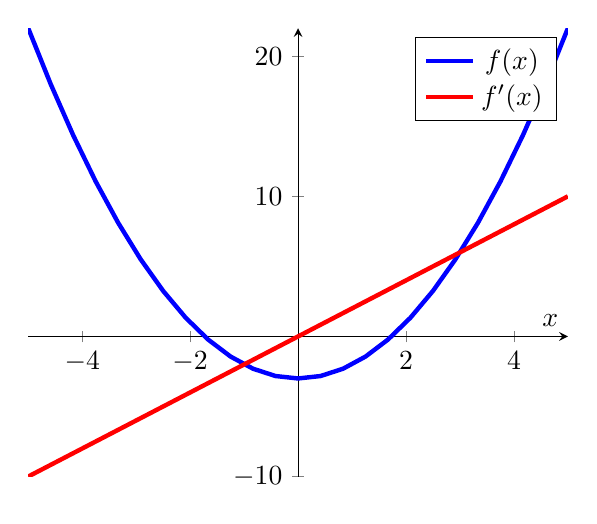
\begin{tikzpicture}
        \begin{axis}[
            axis lines = center,
            xlabel = \(x\)
        ]
        \addplot[blue, ultra thick] {x*x-3};
        \addlegendentry{$f(x)$}
        \addplot[red,  ultra thick] {2*x};
        \addlegendentry{$f'(x)$}
        \end{axis}
    \end{tikzpicture}
    \caption{När funktionen $f(x)$ pekar neråt (sett från vänster till höger) är derivatan $f'(x)$ negativ. Ju mer positiv (uppåt) lutning $f(x)$ har, desto mer positiv blir $f'(x)$.}
    \label{fig:1}
\end{figure}

I figur \ref{fig:1} så är $f(x) = x^2 - 3$ och $f'(x) = 2x$. Målet med det här kapitlet är att lära oss reglerna vi följer när vi tar reda på derivatan av en funktion.

\begin{regel}
    \[f(x) = x^n \imp f'(x) = nx^{n-1}\]
\end{regel}

\begin{exempel}
    Vad är derivatan av $x^3$?\\
    Svar: $f'(x) = 3\cdot x^{3-1} = 3x^2$
\end{exempel}

\begin{uppgifter}
    Derivera följande funktioner:
    \begin{multicols}{3}
        \begin{enumerate}
            \item $f(x) = x^4 \\ f'(x) \ans$
            \item $g(x) = x^2 \\ g'(x) \ans$
            \item $h(x) = x^{27} \\ h'(x) \ans$
        \end{enumerate}
    \end{multicols}
\end{uppgifter}

\subsection{Derivatan av polynom}

\begin{regel}
    \label{reg:kxn}
    \[f(x) = kx^n \imp f'(x) = knx^{n-1}\]
\end{regel}
Som du kanske märkte så ''hände'' det inget med $k$:et. Det är en generell regel -- en siffra multiplicerad med en funktion finns kvar efter att funktionen deriverats. Vi kan formulera den generella regeln så här:

\begin{regel}
    \label{reg:kf(x)}
    \[ f(x) = k g(x) \imp f'(x) = k g'(x) \]
\end{regel}

\begin{exempel}
    Vad är derivatan av $3x^2$? \\ Svar: $f'(x) = 3\cdot 2x^{2-1} = 6x$
\end{exempel}

\begin{uppgifter}
    Derivera följande funktioner:
    \begin{multicols}{3}
        \begin{enumerate}
            \item $f(x) = 3x^4 \\ f'(x) \ans$
            \item $g(x) = 4x^2 \\ g'(x) \ans$
            \item $h(x) = 2x^{27} \\ h'(x) \ans$
        \end{enumerate}
    \end{multicols}
\end{uppgifter}

Vi behöver en till regel för att kunna derivera alla polynom -- vi behöver veta hur vi hanterar funktioner med plustecken i. Som tur är så fungerar det på enklast tänkbara sätt, vi deriverar bara varje term för sig.

\begin{exempel}
    \label{ex:3x2}
    Vad är derivatan av $3x^2 + x^3$? \\ Svar: $f'(x) = 6x + 3x^2$
\end{exempel}

Du kanske ser mönstret utifrån exemplet, här är iallafall den generella regeln:

\begin{regel}
    \label{reg:sum}
    \[ f(x) = g(x) + h(x) \imp f'(x) = g'(x) + h'(x) \] 
\end{regel}

Kolla igen på exempel \ref*{ex:3x2} här ovanför och se att du är med på hur det funkar innan du gör övningsuppgifterna här under.

\begin{uppgifter}
    Derivera följande funktioner:
    \begin{multicols}{3}
        \begin{enumerate}
            \item $f(x) = 3x^4 + 1 \\ f'(x) \ans$
            \item $g(x) = 4x^2 + 3x \\ g'(x) \ans$
            \item $h(x) = 2x^{27} - 3x^3 + x \\ h'(x) \ans$
        \end{enumerate}
    \end{multicols}
\end{uppgifter}

\subsection{Derivatan av $a^x$}
Nu ska vi utvidga till derivator av funktioner där $x$ finns i exponenten, en grupp av funktioner som kallas \emph{exponentialfunktioner.}

Vi har följande regel som gäller för ett speciellt värde, när siffran i basen är $e \approx 2,77$.

\begin{regel}
    \[f(x) = e^x \imp f'(x) = e^x \]
\end{regel}

För en förklaring för vad $e$ är och var regeln kommer från, se Appendix \ref*{app:e} på sidan \pageref*{app:e}.

\begin{uppgifter} 
    Derivera följande funktioner: \\(kom ihåg räkneregel \ref*{reg:kf(x)} på sidan \pageref*{reg:kf(x)}, och räkneregel \ref*{reg:sum} på sidan \pageref*{reg:sum}).
    \begin{multicols}{3}
        \begin{enumerate}
            \item $f(x) = e^x \\ f'(x) \ans$
            \item $g(x) = 3e^x \\ g'(x) \ans$
            \item $h(x) = 2e^x + x^2 \\ h'(x) \ans$
        \end{enumerate}
    \end{multicols}
\end{uppgifter}


\begin{regel}
    \label{reg:e^kx}
    \[ f(x) = e^{kx} \imp f'(x) = ke^{kx} \]
\end{regel}


\begin{exempel}
    Vad är derivatan av $f(x) = e^{3x}$? \\
    Svar: $f'(x) = 3e^{3x}$
\end{exempel}


\begin{exempel}
    Vad är derivatan av $f(x) = \dfrac 1{e^x}$? \\
    Lösning: Vi börjar med att skriva om $f(x)$ med hjälp av potensregler. 
    \[ \frac 1{e^x} = e^{-x} = e^{(-1)x} \]
    Nu kan vi använda räkneregel \ref*{reg:e^kx}. \\
    Svar: $f'(x) = (-1)\cdot e^{(-1)x} = -e^{-x} = -\dfrac 1{e^x}$
\end{exempel}


\begin{uppgifter}
    Derivera följande funktioner:
    \begin{multicols}{3}
        \begin{enumerate}
            \item $f(x) = \dfrac{1}{e^{-3x}} \\ f'(x) \ans$
            \item $g(x) = e^{5x} \\ g'(x) \ans$
            \item $h(x) = 2e^x + \dfrac 1{e^x} - e^{-2x} \\ h'(x) \ans$
        \end{enumerate}
    \end{multicols}
\end{uppgifter}

\subsubsection{Funktionen $a^x$}
Om du tittar på figur \ref*{fig:2^x} på sidan \pageref*{fig:2^x} och figur \ref*{fig:4^x} på sidan \pageref*{fig:4^x} så ser du att derivatan får en faktor framför sig, 1,4 i ena fallet och 0,7 i det andra. Den faktorn är värdet av funktionen $\ln(2)$ för $f(x) = 2^x$ och $\ln(4)$ för $f(x) = 4^x$. Funktionen $\ln (x)$ kallas för den \emph{naturliga logaritmen}, och beskrivs i XXXXXXX.


\begin{regel}
    \label{reg:a^x}
    \[f(x) = a^x \imp f'(x) = \ln (a) a^x \]
\end{regel}


\begin{exempel}
    \label{ex:a^x}
    Vad är derivatan till $3^x$?
    Svar: $f'(x) = \ln (3) 3^x$
\end{exempel}

Vi räknar väldigt sällan ut vad ett tal som $\ln(3)$ blir i decimalform --- om vi inte absolut behöver så är det enklast att låta det stå som det är.

Vi har en till regel för detta som liknar regel \ref*{reg:e^kx} på sidan \pageref*{reg:e^kx}:

\begin{regel}
    \label{reg:a^kx}
    \[f(x) = a^{kx} \imp f'(x) = k\ln(a)a^x\]
\end{regel}


\begin{exempel}
    Vad är derivatan av $f(x) = \dfrac 2{4^{2x}}$?
    
    Lösning: Vi börjar med att skriva om $f(x)$ med hjälp av potensregler.
    \[\dfrac{2}{4^{2x}} = 2\dfrac{1}{4^{2x}} = 2\cdot 4^{-2x} = 2\cdot 4^{(-2)x}\]

    Nu kan vi använda räkneregel \ref*{reg:a^kx}.

    Svar: $f'(x) = 2\cdot (-2) \cdot \ln(4) 4^{-2x} = - \dfrac {4\ln(4)} {4^{2x}}$
\end{exempel}

\begin{uppgifter}
    Derivera följande funktioner:
    \begin{multicols}{3}
        \begin{enumerate}
            \item $f(x) = 3^x \\ f'(x) \ans$
            \item $g(x) = \dfrac{1}{2^{-3x}} \\ g'(x) \ans$
            \item $h(x) = 2\cdot 3^x + \dfrac 2{3^x} - \dfrac 2{-3^x} \\ h'(x) \ans$
        \end{enumerate}
    \end{multicols}
\end{uppgifter}

\newpage

\begin{blu}
    Derivera följande funktioner:
    
    \begin{itemize}
        \begin{tabular}[b]{p{10em} p{20em}}
            \item $f(x) = x^2$  & \item[] $ f'(x) \ans $ \\
            \item $g(x) = \dfrac{1}{x^2} $ & \item[] $g'(x) \ans$ \\
            \item $h(x) = 2\cdot 3^x + 3x^2 $ & \item[] $h'(x) \ans$ \\
            \item $i(x) = 2^x $ & \item[] $i'(x) \ans$\\
            \item $j(x) = e^{-x} - e^x $ & \item[] $j'(x) \ans$\\
            \item $k(x) = \dfrac{4}{3x^2}-e^x + 3 $ & \item[] $k'(x) \ans$\\
            \item $l(x) = x^{13} - 13^x $ & \item[] $ l'(x) \ans$ \\
            \item $m(x) = \dfrac{2}{5\cdot 3^x} $ & \item[] $ m'(x) \ans$ \\
            \item $n(x) = \dfrac{x^5}{5} $ & \item[] $ n'(x) \ans$ \\
            \item $o(x) = e^{x-3} $ & \item[] $ o'(x) \ans$ \\
            \item $p(x) = \dfrac{2^{x+2}}{2^{2(x-2)}}$ & \item[] $ p'(x) \ans$ \\
        \end{tabular}
    
    \end{itemize}
    
\end{blu}


\newpage

\Huge{\textbf{Appendix}}
\normalsize
\appendix

\section{Konstanten $e$ och funktionen $e^x$} 
\label{app:e}
Vi börjar med att studera grafen till funktionen $2^x$.

\begin{figure}[h!]
    \centering
    \begin{mdframed}[backgroundcolor=gray!10]
        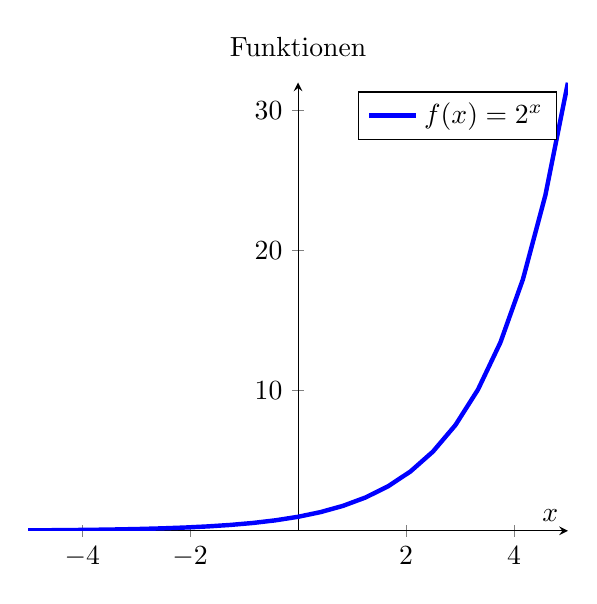
\begin{tikzpicture}
            \begin{axis}[
                axis lines = center,
                xlabel = \(x\),
                ymin = 0,
                ymax = 32,
                title = Funktionen
            ]
            \addplot[blue, ultra thick] {2^x};
            \addlegendentry{$f(x) = 2^x$}
            \end{axis}
        \end{tikzpicture}
        \hskip 5pt
        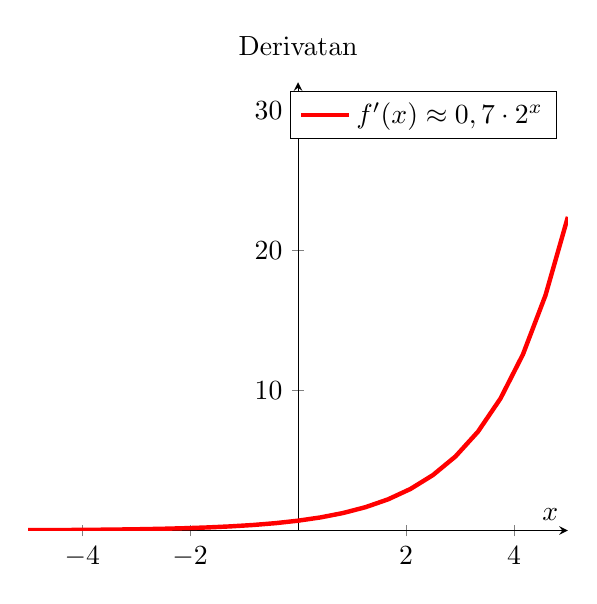
\begin{tikzpicture}
            \begin{axis}[
                axis lines = center,
                xlabel = \(x\),
                ymin = 0,
                ymax = 32,
                title = Derivatan
            ]
            \addplot[red, ultra thick] {0.7*2^x};
            \addlegendentry{$f'(x) \approx 0,7\cdot 2^x$}
            \end{axis}
        \end{tikzpicture}  
        \caption{Exponentialfunktionen $f(x) = 2^x$ till vänster och funktionens derivata till höger.}
        \label{fig:2^x}
        
    \end{mdframed}
\end{figure}

Funktionen har en speciell egenskap: den lutar mer och mer brant ju större värdet blir. Det verkar som att \emph{derivatan} av $2^x$ ökar samtidigt som funktionen själv ökar. Om vi testar med funktionen $f(x) = 4^x$ så får vi ett liknande samband --- men denna gång åt andra hållet, derivatan är lite större än funktionen.

\begin{figure}[h!]
    \centering
    \begin{mdframed}[backgroundcolor=gray!10]
        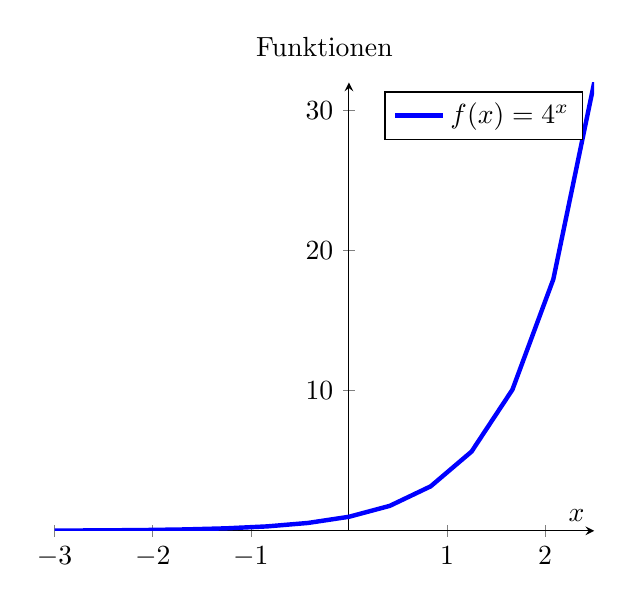
\begin{tikzpicture}
            \begin{axis}[
                axis lines = center,
                xlabel = \(x\),
                ymin = 0,
                ymax = 32,
                xmin = -3,
                xmax = 2.5,
                title = Funktionen
            ]
            \addplot[blue, ultra thick] {4^x};
            \addlegendentry{$f(x) = 4^x$}
            \end{axis}
        \end{tikzpicture}
        \hskip 5pt
        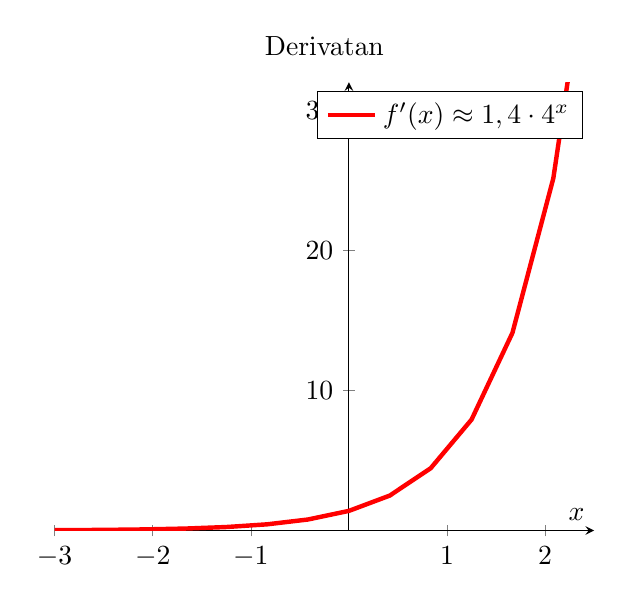
\begin{tikzpicture}
            \begin{axis}[
                axis lines = center,
                xlabel = \(x\),
                ymin = 0,
                ymax = 32,
                xmin = -3,
                xmax = 2.5,
                title = Derivatan
            ]
            \addplot[red, ultra thick] {1.4*(4^x)};
            \addlegendentry{$f'(x) \approx 1,4\cdot 4^x$}
            \end{axis}
        \end{tikzpicture}
        \caption{Exponentialfunktionen $f(x) = 4^x$ till vänster och funktionens derivata till höger.}
        \label{fig:4^x}
    \end{mdframed}
\end{figure}

De två graferna liknar varandra --- men de är inte helt likadana. Det finns ett värde vi kan stoppa in istället för 2 eller 4 som gör att $f(x)$ och $f'(x)$ är exakt likadana --- en funktion som är sin egen derivata. Den funktionen är $e^x$, och $e$ är en konstant, $e\approx 2,72$.

\begin{figure}[h!]
    \centering
    \begin{mdframed}[backgroundcolor=gray!10]
        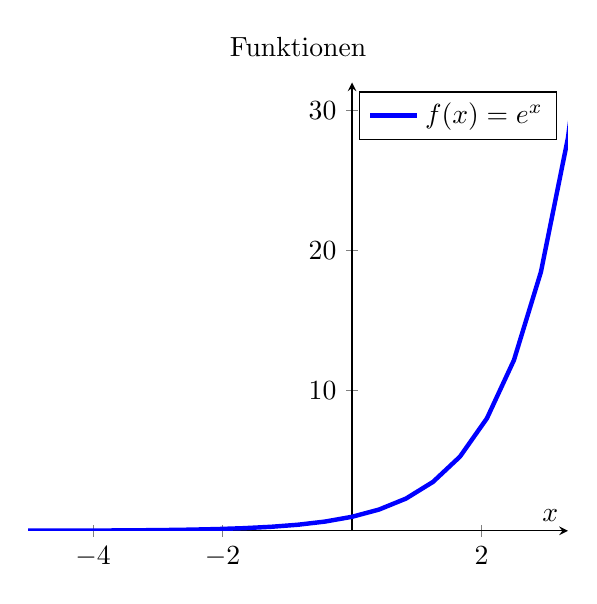
\begin{tikzpicture}
            \begin{axis}[
                axis lines = center,
                xlabel = \(x\),
                ymin = 0,
                ymax = 32,
                title = Funktionen
            ]
            \addplot[blue, ultra thick] {e^x};
            \addlegendentry{$f(x) = e^x$}
            \end{axis}
        \end{tikzpicture}
        \hskip 5pt
        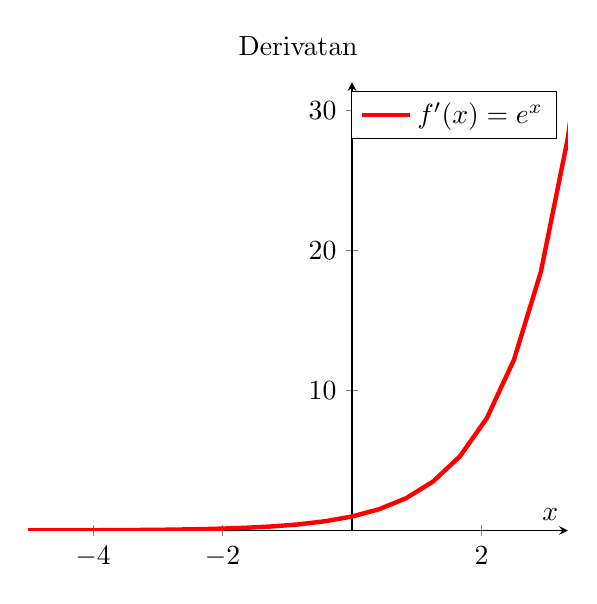
\begin{tikzpicture}
            \begin{axis}[
                axis lines = center,
                xlabel = \(x\),
                ymin = 0,
                ymax = 32,
                title = Derivatan
            ]
            \addplot[red, ultra thick] {e^x};
            \addlegendentry{$f'(x) = e^x$}
            \end{axis}
        \end{tikzpicture}
        \caption{Exponentialfunktionen $f(x) = e^x$ till vänster och funktionens derivata till höger.}
        \label{fig:e^x}
    \end{mdframed}
\end{figure}

Vi har hittat $ e \approx 2.77$, en siffra som ger oss den här väldigt användbara regeln:

\begin{regel}
    \[f(x) = e^x \imp f'(x) = e^x \]
\end{regel}

\end{document}